The assembly of the structure involves the integration of the array of all the actuators, the platform on which they are mounted, and the electronics responsible for controlling the linear actuators. The components of the platform are illustrated in Figure \ref{fig:platform-assembly}, and the corresponding parts list is provided in Table \ref{tab:platform-assembly}. The structure features a hexagonal in a shape, with includes only three lateral structural supports, made of acrylic, and the upper and lower bases, also made of acrylic. The aforementioned components are connected using 3D printed L-shaped joints. A void is present beneath the actuators, with dimensions to approximately 25 cm, to accommodate the rods.


\begin{figure}[!hbt]
    \centering
    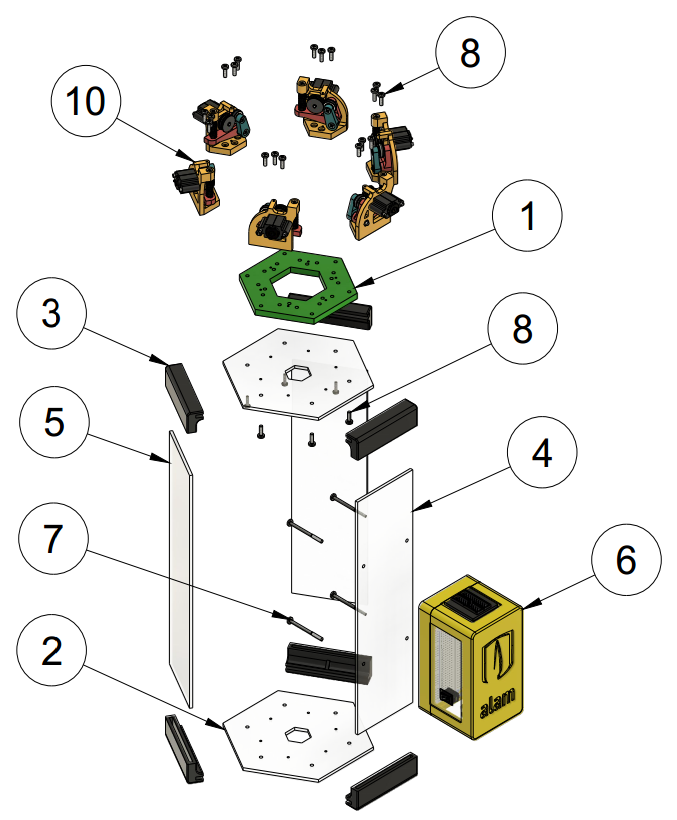
\includegraphics[width=0.7\textwidth]{platform-assembly}
    \caption{Platform assembly exploded-view}
    \label{fig:platform-assembly}
\end{figure}
\begin{table}[!hbt]
    \centering
    \caption{Platform assembly parts list}
    \label{tab:platform-assembly}
    \begin{tabular}{llll}
    \toprule
    Item & Qty & Part Name / Description & Source \\
    \midrule
    1 & 1 & Actuators Base & 3D Printed \\
    2 & 2 & Support Base & Acrylic Laser Cut \\
    3 & 6 & Support Union & Acrylic Laser Cut \\
    4 & 1 & Support Front & Acrylic Laser Cut \\
    5 & 2 & Support Lateral & Acrylic Laser Cut \\
    6 & 1 & Electronics Assembly & \\
    7 & 4 & Binding Head Screw JIS B 1111 - M3x40 & Commercial \\
    8 & 24 & Binding Head Screw JIS B 1111 - M3x10 & Commercial \\
    9 & 6 & Actuator Assembly & \\
    \bottomrule
    \end{tabular}
\end{table}


\section{Electronics Case}

The electronics case contains all the electronic components that are necessary for the control of the motors. The module is an independent component that can be removed and replaced without disturbing the platform structure. It is conveniently positioned next to the platform for easy access. The case contains the microcontroller unit (MCU), the breadboard on which the motor drivers and various connections are made, as well as the input and output peripherals of the module. These can be seen in Figure \ref{fig:electronics-assembly} and are listed in Table \ref{tab:electronics-assembly}. The housing is 3D printed and consists of two main parts: one containing the MCU and the other containing the breadboard. The peripherals are affixed to the walls, which are constructed from laser-cut acrylic sheets.

\begin{figure}[H]
    \centering
    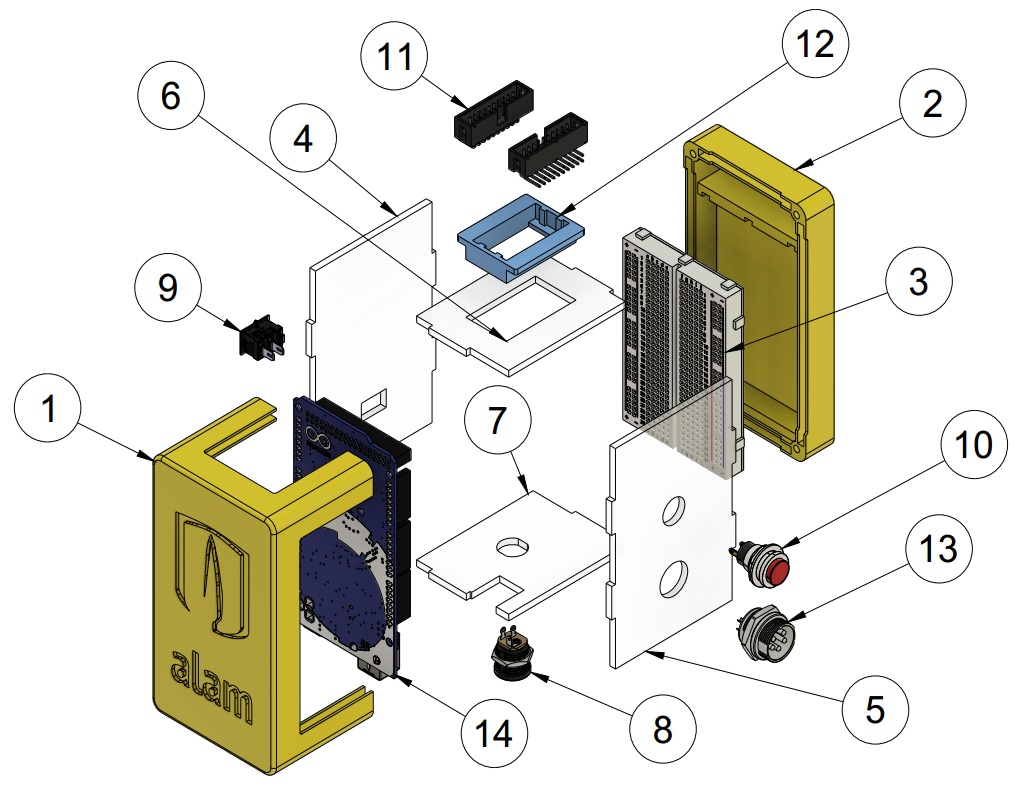
\includegraphics[width=0.9\textwidth]{electronics-assembly}
    \caption{Electronics assembly exploded-view}
    \label{fig:electronics-assembly}
\end{figure}

\begin{table}[h]
    \centering
    \caption{Electronics assembly parts list}
    \label{tab:electronics-assembly}
    \begin{tabular}{llll}
    \toprule
    Item & Qty & Part Name / Description & Source \\
    \midrule
    1 & 1 & Arduino Case & 3D Printed \\
    2 & 1 & Breadboard Base & 3D Printed \\
    3 & 1 & Half-Size Breadboard & Commercial \\
    4 & 1 & Left Wall & Acrylic Laser Cut \\
    5 & 1 & Right Wall & Acrylic Laser Cut \\
    6 & 1 & Top Wall & Acrylic Laser Cut \\
    7 & 1 & Bottom Wall & Acrylic Laser Cut \\
    8 & 1 & DC Power Input Jack - DS-223B & Commercial \\
    9 & 1 & Power Switch - KCD1-11-2P & Commercial \\
    10 & 1 & Red Push Button - DS 212 & Commercial \\
    11 & 2 & IDC 3020-20-0200-00 - 20P 2.54MM & Commercial \\
    12 & 1 & IDC Support & 3D Printed \\
    13 & 1 & MX M12 5-Pin Male MIC Connector Plug & Commercial \\
    14 & 1 & Arduino MEGA 2650 & Commercial \\
    \bottomrule
    \end{tabular}
\end{table}

Figure \ref{fig:electronics-ports} illustrates the ports and connections of the case. The lower section comprises a serial port for programming the MCU and sending commands, as well as a power plug. The right side features an emergency button to prevent the robot from  moving, and a 5-pin connector input for connecting a joystick. The left side houses the power button, while the upper section includes a pair of 20-pin IDC inputs for connecting the unit to the motors.

\begin{figure}
    \centering
    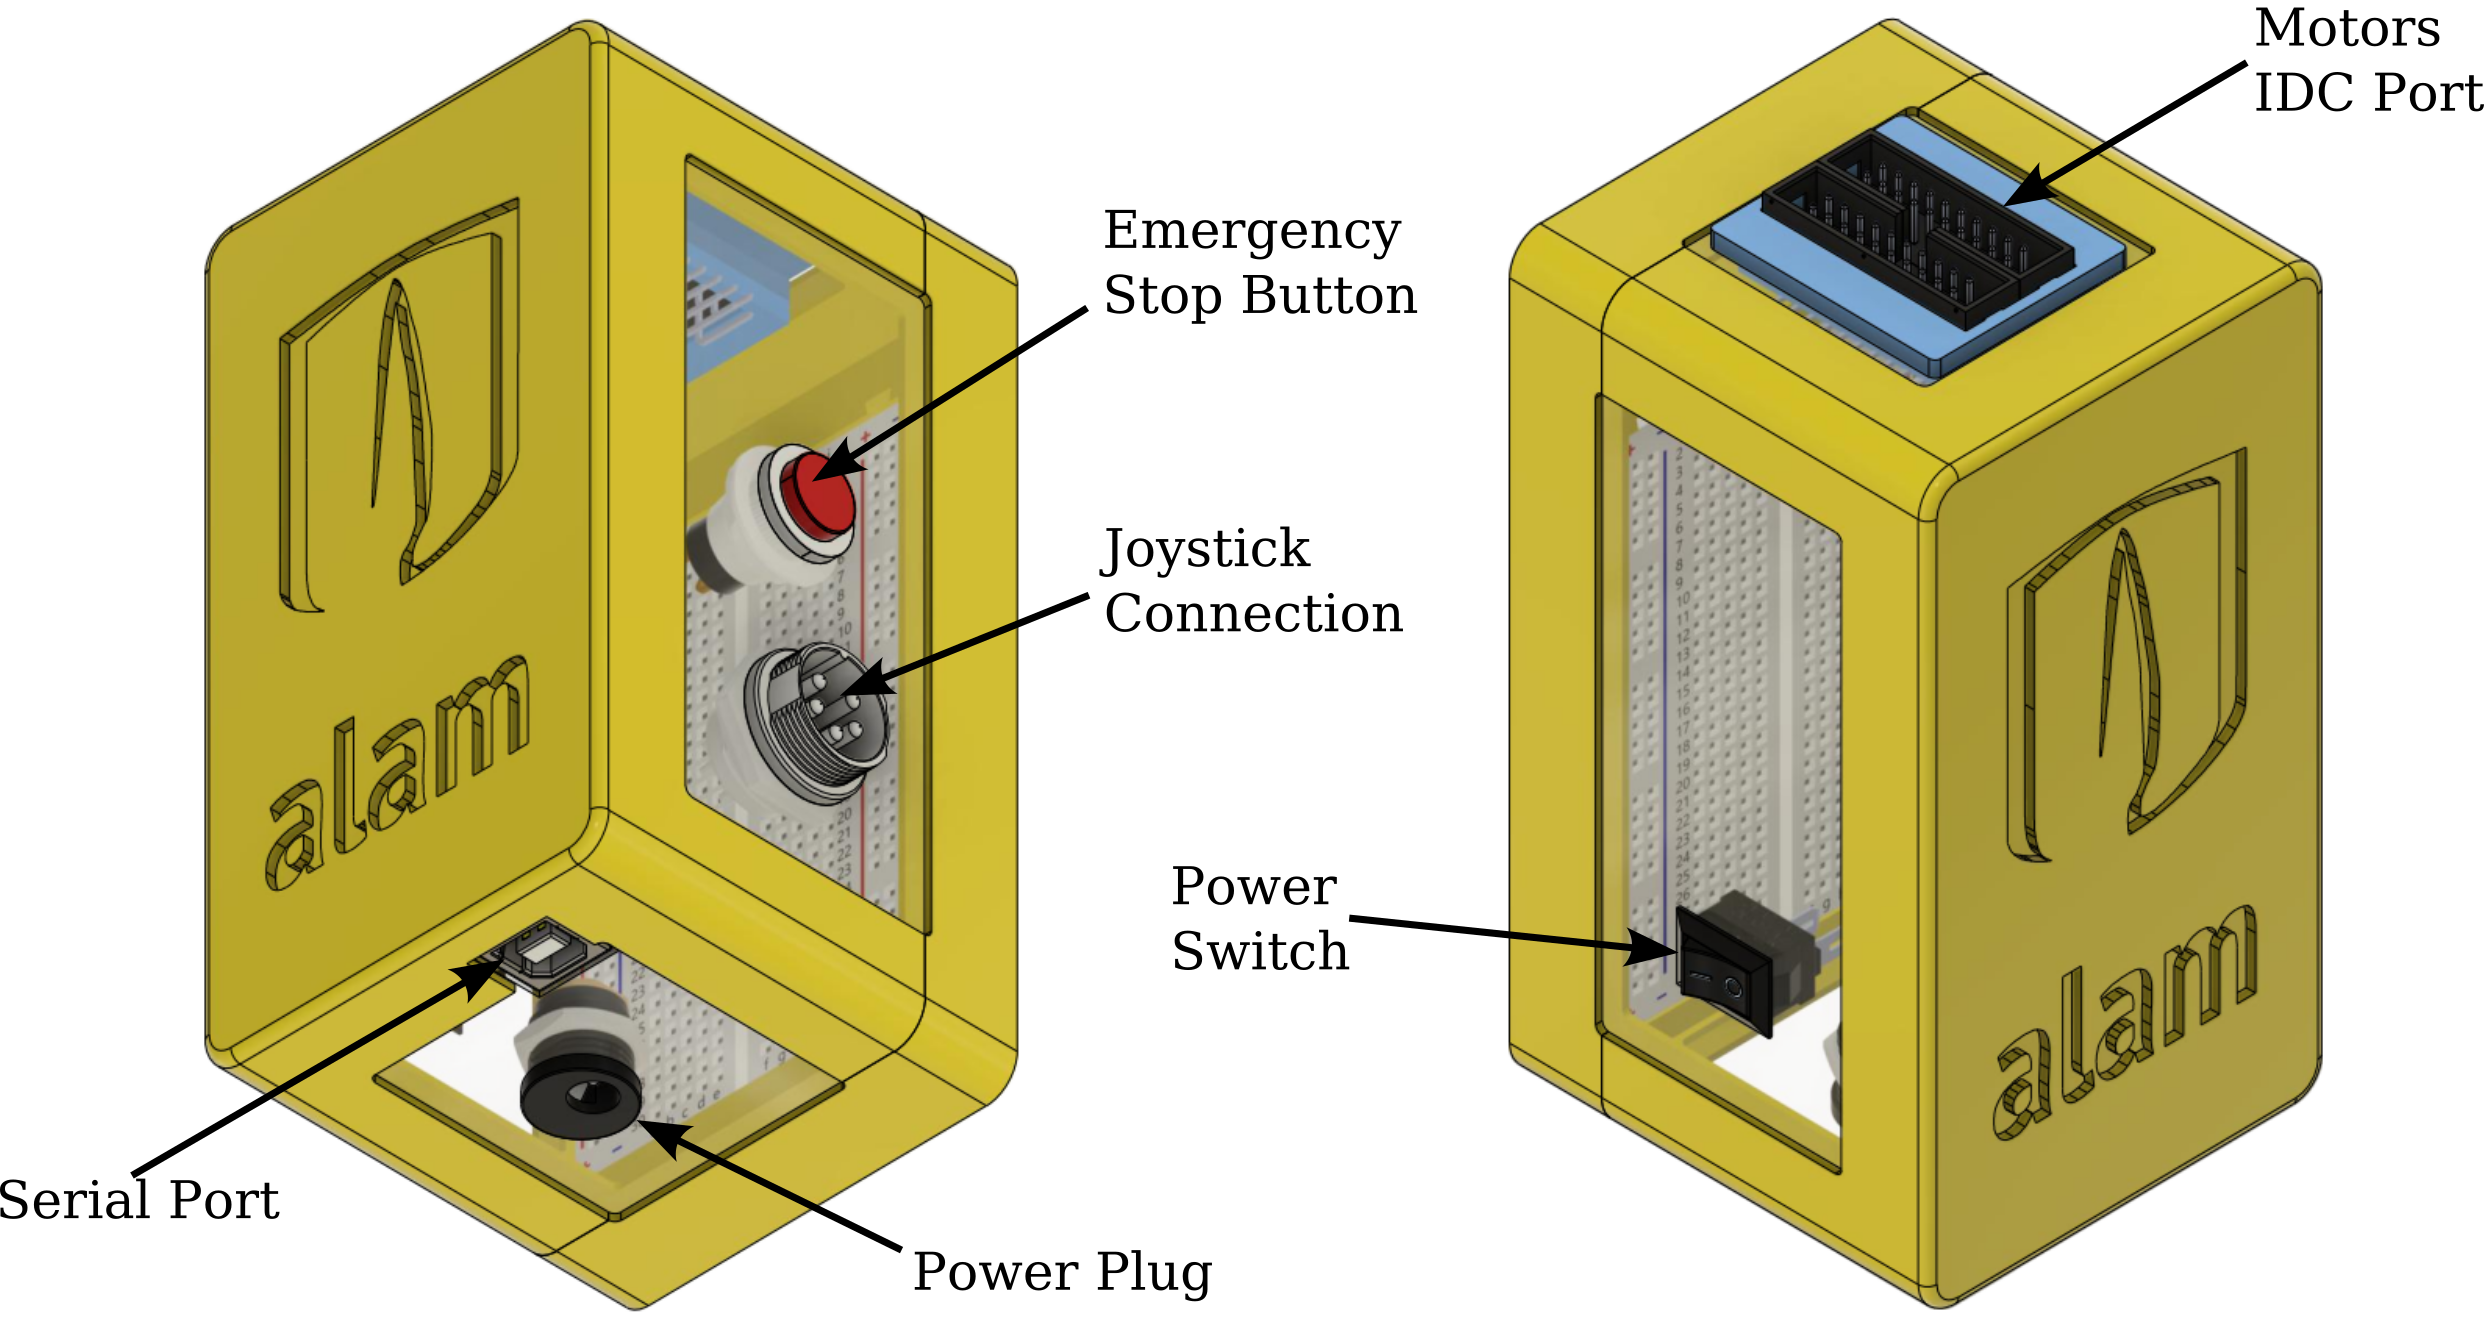
\includegraphics[width=0.85\textwidth]{electronics-ports}
    \caption{Ports and connections}
    \label{fig:electronics-ports}
\end{figure}

\subsection{Circuit Schematic}
The schematic of the circuit connections is illustrated in Figure \ref{fig:main-circuit}. As shown in Figure \ref{fig:motor-circuit}, each actuator motor necessitates six connections. The pins designated as \texttt{M1} and \texttt{M2} are responsible for supplying power to the motors, while the pins designated as \texttt{VCC} and \texttt{GND} provide power to the magnetic encoder. The pins \texttt{A} and \texttt{B} are utilized for quadrature output.

In order to accurately count the encoder pulses in both directions, it is necessary to connect one pin to an interrupt pin and the other to a digital pin. The motor driver, designated as \texttt{DRV8833}, is employed to regulate the polarity and speed of the motors. This device necessitates two PWM connections for each motor. In view of the necessity for a cost-effective MCU with an adequate number of pins to connect six motors, the \texttt{Arduino MEGA 2650} was selected for this project.

\begin{figure}
    \centering
    \includesvg[width=\textwidth]{main-connection2}
    \caption{Main circuit schematic}
    \label{fig:main-circuit}
\end{figure}

\begin{figure}
    \centering
    \includesvg[width=\textwidth]{motor-connection2}
    \caption{Motor circuit schematic}
    \label{fig:motor-circuit}
\end{figure}
